\subsubsection{Q10.20 data 10312021 11092021 grouped by scenario \& x_first}

\begin{comment}
                     EFPR        EO      EFNR     n    pvalue
(frauth, False)  0.437500  0.562500  0.416667  24.0  0.504036
(frauth, True)   0.552632  0.447368  0.500000  19.0  0.533114
(icu, False)     0.468750  0.531250  0.656250  16.0  0.396605
(icu, True)      0.725000  0.275000  0.600000  20.0  0.020688
(rent, False)    0.305556  0.694444  0.444444  18.0  0.019016
(rent, True)     0.476190  0.523810  0.523810  21.0  0.971474
\end{comment}

\begin{table}[h]
    \centering
    \begin{tabular}{|c|c|c|c|c|c|c|}
        \hline
        scenario & x_first & EFPR & EO & EFNR & n & p-value\\
        \hline
        frauth & False & 0.438 & \textbf{0.562} & 0.417 & 24.0 & 0.504\\
		frauth & True & \textbf{0.553} & 0.447 & 0.500 & 19.0 & 0.533\\
		icu & False & 0.469 & \textbf{0.531} & \textbf{0.656} & 16.0 & 0.397\\
		icu & True & \textbf{0.725} & 0.275 & \textbf{0.600} & 20.0 & \textbf{0.021}\\
		rent & False & 0.306 & \textbf{0.694} & 0.444 & 18.0 & \textbf{0.019}\\
		rent & True & 0.476 & \textbf{0.524} & \textbf{0.524} & 21.0 & 0.971\\
		
        \hline
    \end{tabular}
    \caption{Grouped by scenario x_first}
    \label{tab:my_label}
\end{table}
\begin{figure}[h]
    \centering
    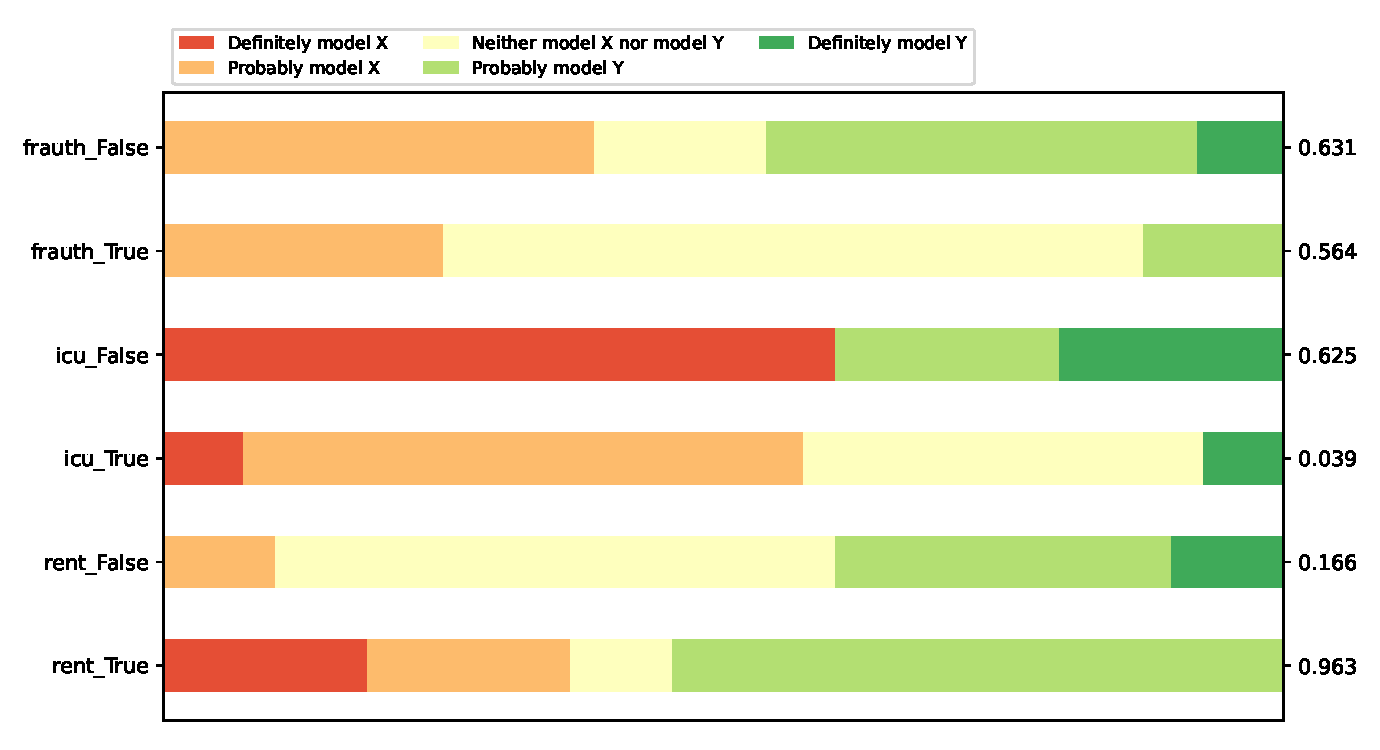
\includegraphics[width=0.8\textwidth]{figures/Q10.20/10312021_11092021/Q10.20_scenario_x_first.pdf}
    \caption{Grouped by scenario \& x_first}
    \label{fig:my_label}
\end{figure}
